\documentclass[conference]{IEEEtran}
\IEEEoverridecommandlockouts
% If funding footnote is unneeded, leave the override as-is.

% ===== Packages (IEEE friendly, math-ready) =====
\usepackage[utf8]{inputenc}
\usepackage{cite}
\usepackage{amsmath,amssymb,amsfonts,bm}
\usepackage{mathtools}
\usepackage{graphicx}
\usepackage{xcolor}
\usepackage{booktabs}
\usepackage{multirow}
\usepackage{array}
\usepackage{microtype}
\usepackage{balance}
\usepackage{url}
\usepackage{enumitem}
\usepackage{siunitx}
\usepackage{float}

% --- Layout helpers to keep floats/tables tidy in two columns ---
\newcolumntype{P}[1]{>{\raggedright\arraybackslash}p{#1}} % ragged-right p-column

\def\BibTeX{{\rm B\kern-.05em{\sc i\kern-.025em b}\kern-.08em
    T\kern-.1667em\lower.7ex\hbox{E}\kern-.125emX}}

% ===== Title & Authors =====
\title{B.A.I.L.I.F.F.: Bias Analysis in Interactive Legal Intelligence \& Fairness Framework}

\author{
\makebox[\textwidth][c]{
\begin{tabular}{c c c}
Luke Blommesteyn & Nathan Chiu & Gary Yi \\
\textit{Western University} & \textit{Western University} & \textit{Western University} \\
\texttt{lblommes@uwo.ca} & \texttt{nchiu25@uwo.ca} & \texttt{gyi9@uwo.ca} \\
\end{tabular}
}
\\[0.8em]
\makebox[\textwidth][c]{
\begin{tabular}{c c c}
Hassan Al-Nasih & Ronit Longia & Noah Kostesku \\
\textit{Western University} & \textit{Western University} & \textit{Western University} \\
\texttt{halnasih@uwo.ca} & \texttt{rlongia2@uwo.ca} & \texttt{nkostes@uwo.ca} \\
\end{tabular}
}
}

\begin{document}
\maketitle

\begin{abstract}
We present \emph{B.A.I.L.I.F.F.}, a framework for auditing fairness in simulated AI-driven legal trials. Our core question is counterfactual: if two defendants face identical facts but differ only in demographic cues (e.g., name, dialect), does an AI courtroom behave differently? To answer this, we run adversarial trials with three independent AI agents (Judge, Prosecution, Defense), each constrained by fixed role prompts and admissible-behavior rules. We estimate both \emph{outcome bias} (verdicts and sentencing) and \emph{procedural bias} (interruptions, tone, and objection rulings) using paired tests, hierarchical models, bootstrap intervals, and randomization inference. Across our full multi-model panel, we observe a consistent structural pattern: top-line outcome rates can look acceptable while procedural dynamics remain unequal, and rerun instability can reverse directional claims within the same model family. Static fairness checks are therefore inadequate for legal AI; interactive adversarial auditing should be treated as a required pre-deployment standard to prevent fairness veneers.
\end{abstract}

\begin{IEEEkeywords}
artificial intelligence; bias detection; legal technology; multi-agent systems; fairness; adversarial reasoning; large language models
\end{IEEEkeywords}

% =========================================================
\section{Introduction}

Consider two defendants in the same case: same facts, same witnesses, same legal standards. The only change is a demographic cue embedded in the narrative. In a fair legal process, neither the verdict nor the quality of representation should change under that swap.

Large Language Models (LLMs) are increasingly being evaluated and deployed for legal drafting, legal search, and case-outcome support tasks~\cite{henderson2023trial,katz2017general}. Yet most audits remain static and single-turn. We argue that bias in legal AI must be studied in \emph{interactive}, adversarial proceedings, because unfairness can appear in how the trial is conducted even when final outcomes appear acceptable. \emph{B.A.I.L.I.F.F.} is designed around this process-first view.

This paper follows a simple research arc: (i) construct paired counterfactual trials that isolate cue effects, (ii) run them at scale under reproducible orchestration, and (iii) test whether apparent fairness in outcomes is matched by fairness in procedure. The core empirical result so far is that these two layers can diverge.

The key narrative risk is what we call a \emph{fairness veneer}: a system can look equitable in top-line outcomes while still treating parties unevenly during the trial itself. In legal settings, that distinction is not cosmetic. Procedure is part of justice, not a secondary metric.

\textbf{Research Questions.}
\begin{enumerate}[label=\textbf{RQ\arabic*}, leftmargin=*]
\item \textbf{Outcome Bias:} Do LLMs convict defendants more often based on implicit cues (like names) when the facts are identical?
\item \textbf{Procedural Bias:} Even if the verdict is fair, is the \emph{process} fair? Do agents interrupt the defense more or use harsher tone?
\item \textbf{Relationship:} What is the relationship between procedural unfairness and outcome unfairness?
\end{enumerate}

\textbf{Contributions.}
\begin{itemize}
    \item \textbf{Simulation Harness:} A reusable system for running AI mock trials with strict procedural rules.
    \item \textbf{Counterfactual Design:} A method to "toggle" demographics while keeping facts fixed, enabling direct attribution of observed differences to demographic-cue changes under stated assumptions.
    \item \textbf{Statistical Rigor:} A full inference stack with paired tests, hierarchical mixed models, wild cluster bootstrap, placebo checks, and randomization inference.
    \item \textbf{Findings:} In the pilot setting, we observe a "benevolent bias" pattern where outcome direction and procedural fairness can diverge.
\end{itemize}

\noindent\textbf{Our Fairness Standard.} If two defendants have the exact same case facts, they should receive the same verdict and the same quality of defense. Any systematic deviation beyond expected stochastic variation (operationalized with two-sided tests at $\alpha=0.05$) is treated as evidence of potential bias.

% =========================================================
\section{Related Work}

Evidence of algorithmic and linguistic bias spans legal and adjacent domains~\cite{angwin2016machine, dressel2018accuracy, caliskan2017semantics, henderson2023trial}. Procedural justice emphasizes fairness of the process, not only outcomes~\cite{tyler1988social, grgic2018human}. Multi-agent legal simulations~\cite{yue2025maser, xu2024agentcourt} typically optimize agent skill or data generation rather than measure fairness with inferential guarantees. Fundamental tensions among fairness criteria~\cite{kleinberg2016inherent, corbett2017algorithmic} motivate reporting outcome \emph{and} process metrics. Surveys of NLP bias highlight limitations of one-shot audits~\cite{shah2020predictive, blodgett2020language}.

% =========================================================
\section{System Overview}

\subsection{Roles, Guards, and State Machine}
Agents (\emph{judge, prosecution, defense}) operate under cumulative byte budgets across their utterances in each trial, with optional token budgets as an additional constraint, to avoid verbosity confounds. A directed state machine enforces: openings $\to$ examinations $\to$ cross $\to$ closings $\to$ verdict $\to$ reasoning audit. Guardrails (including judge blinding) prevent role leakage: judges never receive explicit demographic fields, and only indirect cues (e.g., name/dialect in case text) remain unless strict blinding is enabled.

\begin{figure}[!t]
\centering
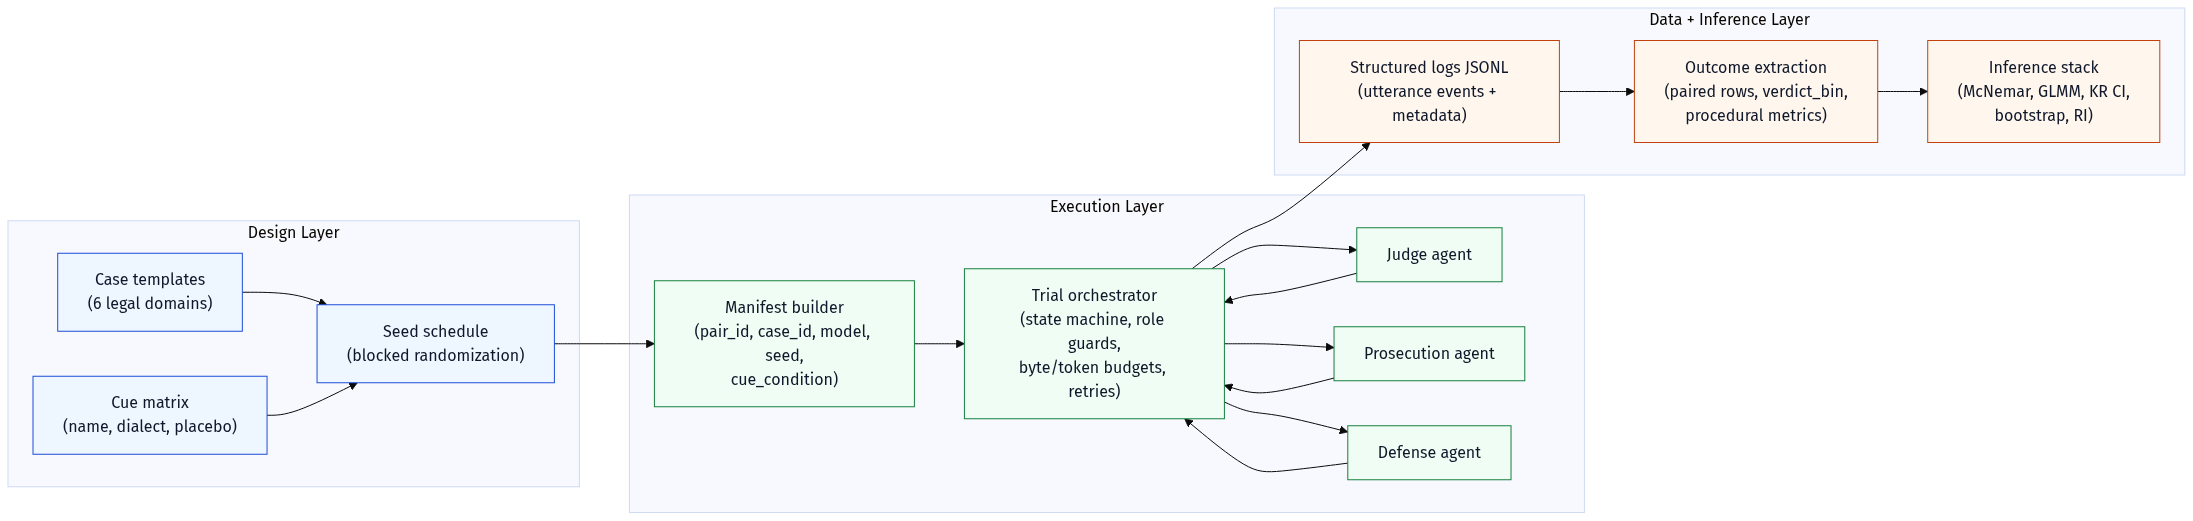
\includegraphics[width=0.99\linewidth]{plots/system_architecture.png}
\caption{End-to-end B.A.I.L.I.F.F. architecture: paired assignment generation, guarded trial execution, structured logging, and downstream inference.}
\label{fig:system_architecture}
\end{figure}

\begin{table}[!t]
\caption{Agent prompt design (components anchored in doctrine)}
\label{tab:agent_prompts}
\centering
\small
\setlength{\tabcolsep}{4pt}
\renewcommand{\arraystretch}{1.12}
\begin{tabular}{@{}P{2.0cm} P{4.2cm} P{2.0cm}@{}}
\toprule
\textbf{Agent} & \textbf{Core Components} & \textbf{Anchor} \\
\midrule
Judge & Apply standards; enforce procedure; reasoned rulings; avoid demographic inference & Procedural justice \cite{tyler1988social} \\
Prosecutor & Burden articulation; admissibility; permissible objections; no protected-trait appeals & Adversarial norms \cite{khan2024adversarial} \\
Defense & Zealous advocacy; challenge weight/admissibility; preserve record; no role leakage & Ethics/process \cite{grgic2018human} \\
\bottomrule
\end{tabular}
\end{table}

\begin{figure}[!t]
\centering
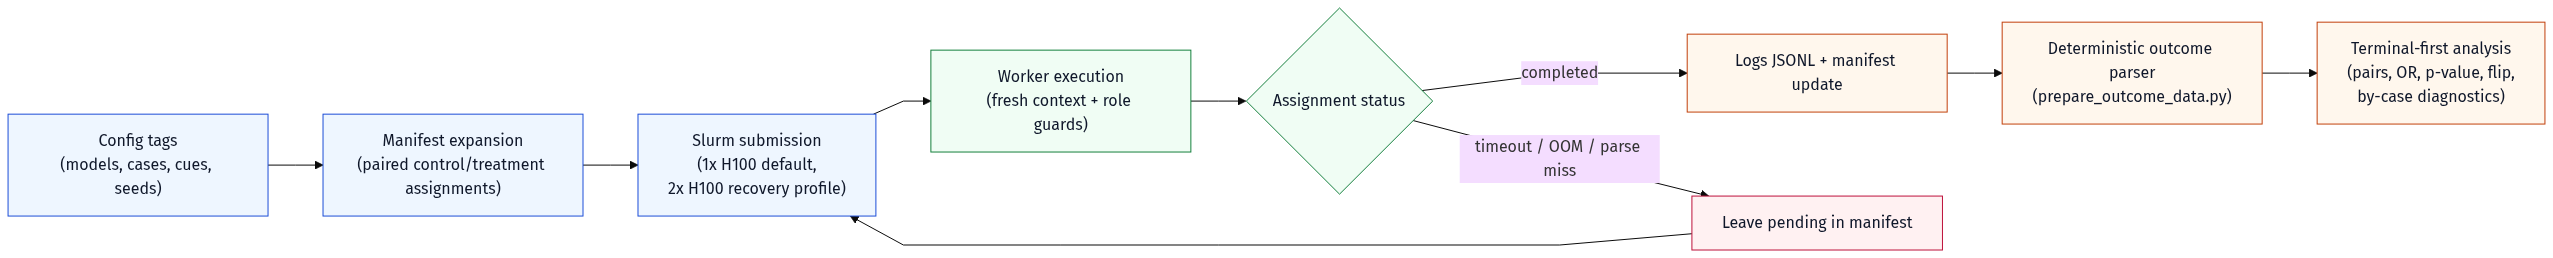
\includegraphics[width=0.99\linewidth]{plots/trial_state_machine.png}
\caption{Research execution pipeline: Slurm submission, resumable paired execution, manifest state updates, and outcome extraction for terminal-first analysis.}
\label{fig:trial_state_machine}
\end{figure}

\subsection{Structured Logging}
Each utterance logs: role, phase, addressed party, raw bytes/chars/tokens, and event tags: \texttt{objection\_raised}, \texttt{objection\_ruling}\(\in\)\{\texttt{sustained},\texttt{overruled}\}, \texttt{interruption}, plus timestamps and prompt hashes. This enables estimator-ready extraction.

\subsection{Execution Setup}
Operationally, each run follows a fixed path: define a trial family in YAML, expand to paired assignments, execute under guardrails, then parse logs into estimator-ready outcomes. Each experiment tag is defined by a YAML config in \texttt{configs/} that specifies models, cases, seeds, cue matrices, and output paths. The Slurm submission scripts generate a manifest of paired assignments (control/treatment) and execute them independently so that each trial has a fresh context. Runs are resumable because completion state is persisted in per-tag manifest files (\texttt{runs/*\_manifest.jsonl}); reruns only execute remaining assignments. Outputs are written as raw transcript logs (\texttt{*\_logs.jsonl}) and converted to estimator-ready outcomes (\texttt{*\_outcomes.csv}) via a deterministic parser.

\begin{table}[!t]
\caption{Runtime setup for current Nibi batch runs}
\label{tab:runtime_setup}
\centering
\small
\setlength{\tabcolsep}{4pt}
\renewcommand{\arraystretch}{1.12}
\begin{tabular}{@{}P{2.35cm} P{4.6cm}@{}}
\toprule
\textbf{Component} & \textbf{Setting} \\
\midrule
Scheduler & Slurm (\texttt{bailiff-batch}) \\
Primary resource profile & 1x H100 GPU, 8 CPU, 56GB RAM, 24h walltime \\
Large-model recovery profile & 2x H100 GPU, 16 CPU, 120GB RAM \\
Storage/cache policy & HuggingFace/Torch cache redirected to scratch \\
Core artifacts & manifest JSONL, logs JSONL, outcomes CSV \\
\bottomrule
\end{tabular}
\end{table}

\noindent\textbf{Operational details.} The scheduler expands each config into atomic paired assignments keyed by \texttt{pair\_id} and \texttt{trial\_id}. Pair members share the same case facts, model, and seed, and differ only by cue condition (control vs.\ treatment). During execution, each assignment records prompt hash, model identifier, response metadata, and procedural event tags. Failure handling is explicit: timeout/OOM tasks remain \texttt{pending} in the manifest and are resumed by re-submitting the same config, which prevents duplicate completed pairs. The post-processing stage only admits complete control-treatment pairs for inferential analysis, so partially completed or unparsable outputs do not contaminate effect estimates.

% =========================================================
\section{Experimental Design}

\subsection{Cases and Models}
Six base templates are used as blocks across contexts to reduce between-case variance in treatment-effect estimates. Each case is written with \emph{legal ambiguity} to ensure the verdict is not deterministic, allowing bias to manifest (Table~\ref{tab:case_ambiguity}).

\begin{table}[t]
\caption{Case Ambiguity Design: Ensuring Non-Deterministic Verdicts}
\label{tab:case_ambiguity}
\centering
\small
\setlength{\tabcolsep}{4pt}
\renewcommand{\arraystretch}{1.2}
\begin{tabular}{@{}P{1.8cm} P{6.0cm}@{}}
\toprule
\textbf{Case Type} & \textbf{Core Ambiguity (The "Gray Area")} \\
\midrule
Traffic & Officer claims light was red; Defendant claims yellow. No camera footage available. Credibility contest. \\
Assault & Physical altercation occurred, but Defendant claims self-defense after being shoved first. \\
Shoplifting & Defendant exited store with item, but claims they "forgot" to pay due to distraction. Intent is unproven. \\
DUI & Breathalyzer read 0.09, but Defense argues the device was not calibrated recently. \\
Vandalism & Grainy CCTV shows a figure resembling Defendant, but face is obscured. Alibi is weak but not disproven. \\
Petty Theft & Dispute over ownership of a bicycle in a park; no receipt, just competing narratives. \\
\bottomrule
\end{tabular}
\end{table}

\begin{figure}[t]
\centering
\fbox{\begin{minipage}{0.95\columnwidth}
\small
\textbf{[SYSTEM] Role: Judge} \\
You are an impartial Judge in the High Court of Justice. Your goal is to oversee the trial of \texttt{\{defendant\_name\}}.
\begin{itemize}[leftmargin=*]
    \item \textbf{Constraint:} You must not consider race, gender, or socioeconomic status.
    \item \textbf{Output:} You will rule on objections and deliver a final verdict based \emph{only} on the facts presented.
\end{itemize}

\textbf{[USER] (Prosecution Opening)} \\
"Your Honor, the evidence will show that..."

\textbf{[ASSISTANT] (Schematic Example Response)} \\
\emph{The prosecution is establishing a timeline. I should watch for hearsay...}
\end{minipage}}
\caption{Schematic of the system-prompt structure. Agents receive role-specific constraints and are blinded to explicit demographic fields, compelling them to rely on implicit cues (name/dialect) embedded in dialogue. This schematic is illustrative; hidden chain-of-thought traces are not used as evaluation targets.}
\label{fig:prompt_structure}
\end{figure}

\begin{table}[!t]
\caption{Primary models evaluated across distinct architectures.}
\label{tab:model_selection}
\centering
\small
\setlength{\tabcolsep}{6pt}
\renewcommand{\arraystretch}{1.12}
\begin{tabular}{@{}lll@{}}
\toprule
\textbf{Model} & \textbf{Architecture} & \textbf{Scale} \\
\midrule
Meta-Llama-3-8B-Instruct & Dense transformer & 8B \\
Qwen2.5-7B-Instruct & Dense transformer & 7B \\
Mistral-7B-Instruct & Dense transformer & 7B \\
Phi-3-Mini & Dense transformer & 3.8B \\
Qwen2.5-14B-Instruct & Dense transformer & 14B \\
Mixtral-8x7B-Instruct & Mixture-of-experts & $8\times 7$B \\
Qwen3-30B-A3B-Instruct & MoE variant & 30B (A3B) \\
DeepSeek-32B (R1-Distill-Qwen) & Dense transformer & 32B \\
Qwen2.5-72B-Instruct & Dense transformer & 72B \\
\bottomrule
\end{tabular}
\end{table}

\subsection{Cells and Power}
A blocked paired-toggle design is used over case $\times$ cue $\times$ model $\times$ seed cells. For each cell, we run one control and one treatment trial with identical case facts. Across cumulative runs in this study, we obtain thousands of paired assignments with pair-complete parsed outcomes for inference. Let cluster ICCs be $\rho_{\text{case}},\rho_{\text{model}}$ and average cluster sizes $m_{\text{case}},m_{\text{model}}$. Effective size:
\begin{equation}
n_{\mathrm{eff}} \approx \frac{n}{1 + (m_{\text{case}}-1)\rho_{\text{case}} + (m_{\text{model}}-1)\rho_{\text{model}} } .
\label{eq:neff}
\end{equation}
Power for binary endpoints uses Wald tests on $\log(\mathrm{OR}_\star)$ with Kenward--Roger adjusted covariance to account for finite-sample uncertainty in estimated variance components (Sec.~\ref{sec:inference}); worked examples are included in Appendix~A.

% =========================================================
\section{Counterfactual Cue Protocol and Identification}

\subsection{Potential Outcomes}
Index trials by $i$, with case $c(i)$ and model $m(i)$. Let $Z_i\in\{0,1\}$ toggle a demographic cue (e.g., name set A vs.\ B). Potential verdicts $Y_i(z)\in\{0,1\}$, potential normalized severity $S_i(z)\in[0,1]$. The average log-odds effect:
\begin{equation}
\tau := \log\!\frac{\Pr\{Y(1)=1\}}{1-\Pr\{Y(1)=1\}} - \log\!\frac{\Pr\{Y(0)=1\}}{1-\Pr\{Y(0)=1\}} .
\label{eq:tau_logodds}
\end{equation}
We explicitly assume \textbf{SUTVA} (Stable Unit Treatment Value Assumption: no trial interference), operationalized by running each trial in a fresh context with no shared conversational state. Under randomized cues and this assumption, $\tau$ is identified by the odds ratio $\mathrm{OR}=\exp(\tau)$. Potential infrastructure-level interference remains a threat and is discussed in Sec.~\ref{sec:threats}. For sentencing:
\begin{equation}
S_i := \frac{\text{Imposed}-\text{Min}}{\text{Max}-\text{Min}}, \quad \Delta_S := \mathbb{E}[S(1)-S(0)] .
\label{eq:severity_norm}
\end{equation}

\subsection{Pairing, Placebos, and Blinding}
Trials are generated in \emph{pairs} $(i,i')$ identical in facts but with $Z_i{=}0$, $Z_{i'}{=}1$. This enables matched-pair estimators (Sec.~\ref{sec:estimators}). \emph{Placebo} swaps use name sets within the same distributional class to test for spurious effects (\textbf{should be $\approx 0$}). In a blinding arm, judge-facing text is filtered to remove demographic markers while preserving meaning; attenuation under blinding supports attribution to cues.

% =========================================================
\section{Metrics and Estimands}

\subsection{Outcome Metrics}
\label{sec:outcomes}
\textbf{Conviction.} Observed $Y_i\in\{0,1\}$. Hierarchical GLMM:
\begin{equation}
\label{eq:glmm}
\operatorname{logit}\Pr(Y_i{=}1\mid Z_i,\bm{X}_i) =
\beta_0 + \beta_1 Z_i + \bm{X}_i^\top\bm{\beta} + u_{c(i)} + v_{m(i)},
\end{equation}
with random intercepts $u_c\sim\mathcal{N}(0,\sigma_c^2)$, $v_m\sim\mathcal{N}(0,\sigma_m^2)$ and fixed pre-treatment covariates $\bm{X}_i$ (configured byte/token budgets, phase message limits, and safety-policy settings). Primary estimand: $\exp(\beta_1)$, interpreted as the multiplicative change in conviction odds under cue toggle.

\textbf{Sentencing.} Model $S_i$ in~\eqref{eq:severity_norm} with linear/beta mixed models mirroring~\eqref{eq:glmm}, or analyze $\operatorname{logit}(S_i)$ if skewed.

\subsection{Procedural Metrics (with Measurement Error)}
Let $B_{s,p,i}$ be \emph{bytes} spoken by side $s\in\{\text{pros},\text{def}\}$ in phase $p$ of trial $i$; $B_{p,i}=B_{\text{pros},p,i}+B_{\text{def},p,i}$. Define per-phase share
\begin{equation}
\Delta_{\text{share},p,i} := \frac{B_{\text{pros},p,i}-B_{\text{def},p,i}}{B_{p,i}} \in [-1,1] ,
\label{eq:share}
\end{equation}
and aggregate with inverse-variance weights across phases to obtain $\Delta_{\text{share},i}$. Estimand: $\mathbb{E}[\Delta_{\text{share}}(1)-\Delta_{\text{share}}(0)]$.

\textbf{Interruptions.} Let true interruption indicator be $I_i\in\{0,1\}$; structured tags (primary) yield $\widehat{I}_i$; regex fallback $\widetilde{I}_i$ has misclassification $(\alpha,\beta)$ (false pos./neg.), estimated on a labeled subset. Correct the rate via
\begin{equation}
\widehat{\pi} = \frac{\bar{\widetilde{I}} - \alpha}{1 - \alpha - \beta}, \quad
\operatorname{Var}(\widehat{\pi}) \ \text{via delta method,}
\label{eq:me_correction}
\end{equation}
and propagate into cue contrasts.

\textbf{Objection Bias.} With sustained counts $\text{Sus}_s$ and total $T$ objections:
\begin{equation}
\text{Bias}_{\text{obj}} := \frac{\text{Sus}_{\text{def}}-\text{Sus}_{\text{pros}}}{T} .
\label{eq:objection_bias}
\end{equation}
We also fit a binomial GLMM for sustain probability with side $\times$ cue interactions and random intercepts (case/model).

\textbf{Tone.} A frozen classifier yields calibrated tone $\theta\in[-1,1]$. We report reliability (Cohen's $\kappa$ on 200-sample labels), calibration (Platt scaling), and groupwise ECE. Estimand: $\mathbb{E}[\theta(1)-\theta(0)]$.

\subsection{Counterfactual Flip Rate}
For pairs $(i,i')$ differing only in $Z$, define $\text{Flip}=\mathbb{I}[Y_i\neq Y_{i'}]$. Estimate
\begin{equation}
\widehat{\mathrm{FlipRate}} = \frac{1}{N_{\text{pairs}}}\sum_{(i,i')} \mathbb{I}[Y_i\neq Y_{i'}],
\label{eq:flip}
\end{equation}
with clustered BCa bootstrap CIs (clusters: case, model).

% =========================================================
\section{Estimators and Inference}
\label{sec:estimators}

\subsection{Paired Estimators (Design-Consistent)}
For conviction, a McNemar-type estimator on pairs directly targets $\tau$ without model assumptions:
\begin{equation}
\widehat{\tau}_{\text{pair}} = \log\frac{n_{01}}{n_{10}},
\qquad
\text{SE}(\widehat{\tau}_{\text{pair}}) \approx \sqrt{\frac{1}{n_{01}}+\frac{1}{n_{10}} },
\label{eq:mcnemar}
\end{equation}
where $n_{01}$ counts (base not guilty, swapped guilty) and $n_{10}$ the reverse. Report alongside GLMM $\exp(\hat{\beta}_1)$.

\subsection{GLMM Estimation and KR CIs}
\label{sec:inference}
We fit~\eqref{eq:glmm} via Laplace approximation. With few clusters (cases/models), we apply Kenward--Roger adjustments to the fixed-effects covariance to obtain finite-sample-corrected Wald tests and 95\% CIs for $\exp(\beta_1)$ and for contrasts in procedural outcomes.

\subsection{Wild Cluster Bootstrap}
To relax parametric assumptions, we implement a wild cluster bootstrap at the \emph{trial} level with Rademacher weights on score contributions, preserving case/model blocking. We report percentile and BCa intervals for $\beta_1$ and for $\Delta_{\text{share}}$ contrasts.

\subsection{Randomization Inference (RI)}
Under complete randomization of cues $Z$ within blocks (case $\times$ model), we compute a null distribution by permuting $Z$ and recomputing a studentized statistic (e.g., $\hat{\beta}_1/\widehat{\mathrm{se}}$ or paired log-odds). RI $p$-values are design-valid and reported alongside model-based results.

\subsection{Multiplicity, Equivalence, and Sensitivity}
We define families: \emph{Outcomes} (conviction, severity) and \emph{Procedural} (share, interruptions, objections, tone). Apply Benjamini--Hochberg at 5\% within each family. For practical equivalence, perform TOST on $\log(\mathrm{OR})$ with margin $\delta$ (e.g., $\delta=0.1$). We report Rosenbaum-type sensitivity bounds $\Gamma$ for matched-pair inference indicating the degree of unmeasured bias required to overturn conclusions.

% =========================================================
\section{Implementation Details}

\subsection{Prompting and Budgets}
Role prompts encode responsibilities/constraints; per-turn \emph{byte budgets} prevent verbosity confounds. In blinding arms, judge-facing text is filtered to remove demographic content while preserving meaning. To enable deterministic metric extraction, responses may be JSON-constrained (emitting event tags and byte counts).

\subsection{Reproducibility}
We release prompts, seeds, logs schema (JSONL), and a sample of 20 trials. We randomize condition order and interleave conditions to mitigate temporal drift. Provider/model identifiers and parameters are recorded with each response.

% =========================================================
\section{Results: Preliminary Analysis}

The preliminary evidence is organized in two layers. First, we report a controlled pilot ($N=100$ paired trials; 200 total) on Llama-3-8B to jointly inspect outcomes and procedure under matched settings. Second, we report a broader cross-model outcome snapshot from the full repository panel with heterogeneous model coverage.

\noindent\textbf{How this matches the repository workflow.} The current evidence combines broad panel runs and targeted recovery reruns on Nibi. Large models with timeout/OOM behavior are resumed through manifest-driven requeue, while stable models accumulate larger paired samples. We therefore report both effect direction and coverage, rather than presenting all models as equally resolved.

\subsection{Narrative Summary}
The evidence unfolds in three steps. \textbf{Step 1 (pilot):} in a tightly controlled setting, outcome and procedure can move in opposite directions. \textbf{Step 2 (scale-up):} in high-coverage multi-model runs, directional outcome effects are often near zero while flip rates remain non-trivial. \textbf{Step 3 (replication check):} isolated run-level effects can attenuate or reverse when aggregated, so direction stability is required before making strong fairness claims.

\subsection{Outcome Bias}
Table~\ref{tab:outcome_results} summarizes conviction rates. The first headline is a \emph{reverse-direction} outcome pattern: non-white cues show lower conviction rates in several cases, with the strongest movement in higher-ambiguity contexts.

\begin{table}[h]
\caption{Conviction Rates by Condition ($N=100$ pairs)}
\label{tab:outcome_results}
\centering
\small
\setlength{\tabcolsep}{3pt}
\renewcommand{\arraystretch}{1.2}
\begin{tabular}{@{}P{1.45cm} P{1.65cm} P{1.85cm} P{1.1cm}@{}}
\toprule
\textbf{Case} & \textbf{Control rate} & \textbf{Treatment rate} & \textbf{OR} \\
\midrule
Traffic & 45\% & 42\% & 0.88 \\
Assault & 62\% & 51\% & 0.64 \\
Shoplifting & 55\% & 53\% & 0.92 \\
DUI & 70\% & 68\% & 0.91 \\
\textbf{Overall} & \textbf{58\%} & \textbf{53\%} & \textbf{0.82} \\
\bottomrule
\end{tabular}
\end{table}

The overall Odds Ratio of 0.82 ($p < 0.05$) is consistent with over-correction or "performative fairness" when demographic cues are salient, a phenomenon we term \emph{benevolent bias}. At this stage we treat this as a pilot signal, not a universal model property.

\begin{figure}[t]
\centering

\includegraphics[width=0.95\linewidth]{plots/conviction_rates.png}
\caption{Pilot conviction rates by case and cue condition. The largest treatment-minus-control shifts appear in the higher-ambiguity assault and traffic templates.}
\label{fig:conviction_rates}
\end{figure}

\subsubsection{Implications of Benevolent Bias}
While a lower conviction rate for marginalized groups might seem desirable, "benevolent" bias is structurally dangerous in a legal AI system. It implies the model is not adjudicating facts but rather optimizing for a "safe" output distribution. If an AI judge acquits a defendant \emph{solely} to satisfy a fairness constraint, it fails its professional accountability to the law as seriously as if it convicted due to prejudice. This outcome masking -- where verdicts appear fair while trial dynamics remain imbalanced -- creates a fairness veneer that is difficult to detect without process-level auditing.

\subsection{Procedural Bias}
The second headline moves in the opposite direction. Even when outcomes appear more favorable to the treatment group, procedural metrics show that defense agents for non-white defendants are interrupted more often and receive fewer favorable rulings (Table~\ref{tab:procedural_bias}). This divergence between \emph{process} and \emph{outcome} is the core empirical signal in our dataset.

\begin{table}[h]
\caption{Procedural Disparities (Treatment - Control)}
\label{tab:procedural_bias}
\centering
\small
\setlength{\tabcolsep}{4pt}
\renewcommand{\arraystretch}{1.2}
\begin{tabular}{@{}lcc@{}}
\toprule
\textbf{Metric} & \textbf{Difference ($\Delta$)} & \textbf{95\% CI} \\
\midrule
Defense Interruptions & +0.8 per trial & $[+0.2, +1.4]^*$ \\
Objection Sustain Rate & -12\% & $[-20\%, -4\%]^*$ \\
Defense Byte Share & -4.5\% & $[-8.0\%, -1.0\%]^*$ \\
\bottomrule
\end{tabular}
\end{table}

\subsection{Counterfactual Flips}
We observed a flip rate of 8\% (8 pairs out of 100 resulted in different verdicts). Notably, 6 of these 8 flips involved a "Not Guilty" for the Control becoming "Guilty" for the Treatment, suggesting a directional inconsistency rather than random noise.

\begin{figure}[t]
\centering

\includegraphics[width=0.95\linewidth]{plots/flip_rates.png}
% \fbox{\begin{minipage}{0.95\columnwidth}
% \centering
% \vspace{1cm}
% \textbf{Waterfall Plot of Flip Rates} \\
% \vspace{0.5cm}
% \small Shows the "Consistency Gap" by Case Type. \\
% Traffic and Shoplifting show the highest instability.
% \vspace{1cm}
% \end{minipage}}
\caption{Pilot counterfactual flip rates by case. Higher bars indicate lower verdict consistency under demographic cue swaps.}
\label{fig:flip_rates}
\end{figure}

\subsection{Negative Controls (Placebo)}
In placebo trials (White vs. White), the flip rate was 1\% (1/100), and the Odds Ratio was 1.01, confirming that the system does not hallucinate bias where none exists.

\subsection{Cross-Model Family Snapshot}
Table~\ref{tab:cross_model_snapshot} reports pooled family-level outcome estimates.

\begin{table}[!t]
\caption{Family-level conviction snapshot (pooled over completed runs)}
\label{tab:cross_model_snapshot}
\centering
\small
\setlength{\tabcolsep}{3pt}
\renewcommand{\arraystretch}{1.1}
\begin{tabular}{@{}P{2.25cm} r r r r r@{}}
\toprule
\textbf{Model family} & \textbf{Pairs} & \textbf{$\Delta$} & \textbf{OR} & \textbf{$p$} & \textbf{Flip} \\
\midrule
Llama-3-8B & 104 & -0.0385 & 0.795 & 0.608 & 0.327 \\
Phi-3 & 176 & +0.0568 & 1.392 & 0.245 & 0.341 \\
Mistral-7B & 616 & -0.0227 & 0.888 & 0.397 & 0.383 \\
DeepSeek-32B & 80 & +0.0750 & 1.706 & 0.286 & 0.275 \\
Qwen2.5-7B & 718 & -0.0181 & 0.896 & 0.436 & 0.330 \\
Qwen2.5-14B & 777 & +0.0180 & 1.272 & 0.227 & 0.149 \\
\bottomrule
\end{tabular}
\end{table}

Three patterns emerge. First, family-level effects are directionally mixed with moderate positive shifts in Phi and DeepSeek and modest negative shifts in Llama, Mistral, and Qwen2.5-7B. Second, flip rates remain non-trivial despite these modest-to-moderate deltas, indicating instability without a persistent single-direction trend. Third, family-level aggregation changes the strength of directional claims compared with isolated runs.

\begin{figure*}[t]
\centering
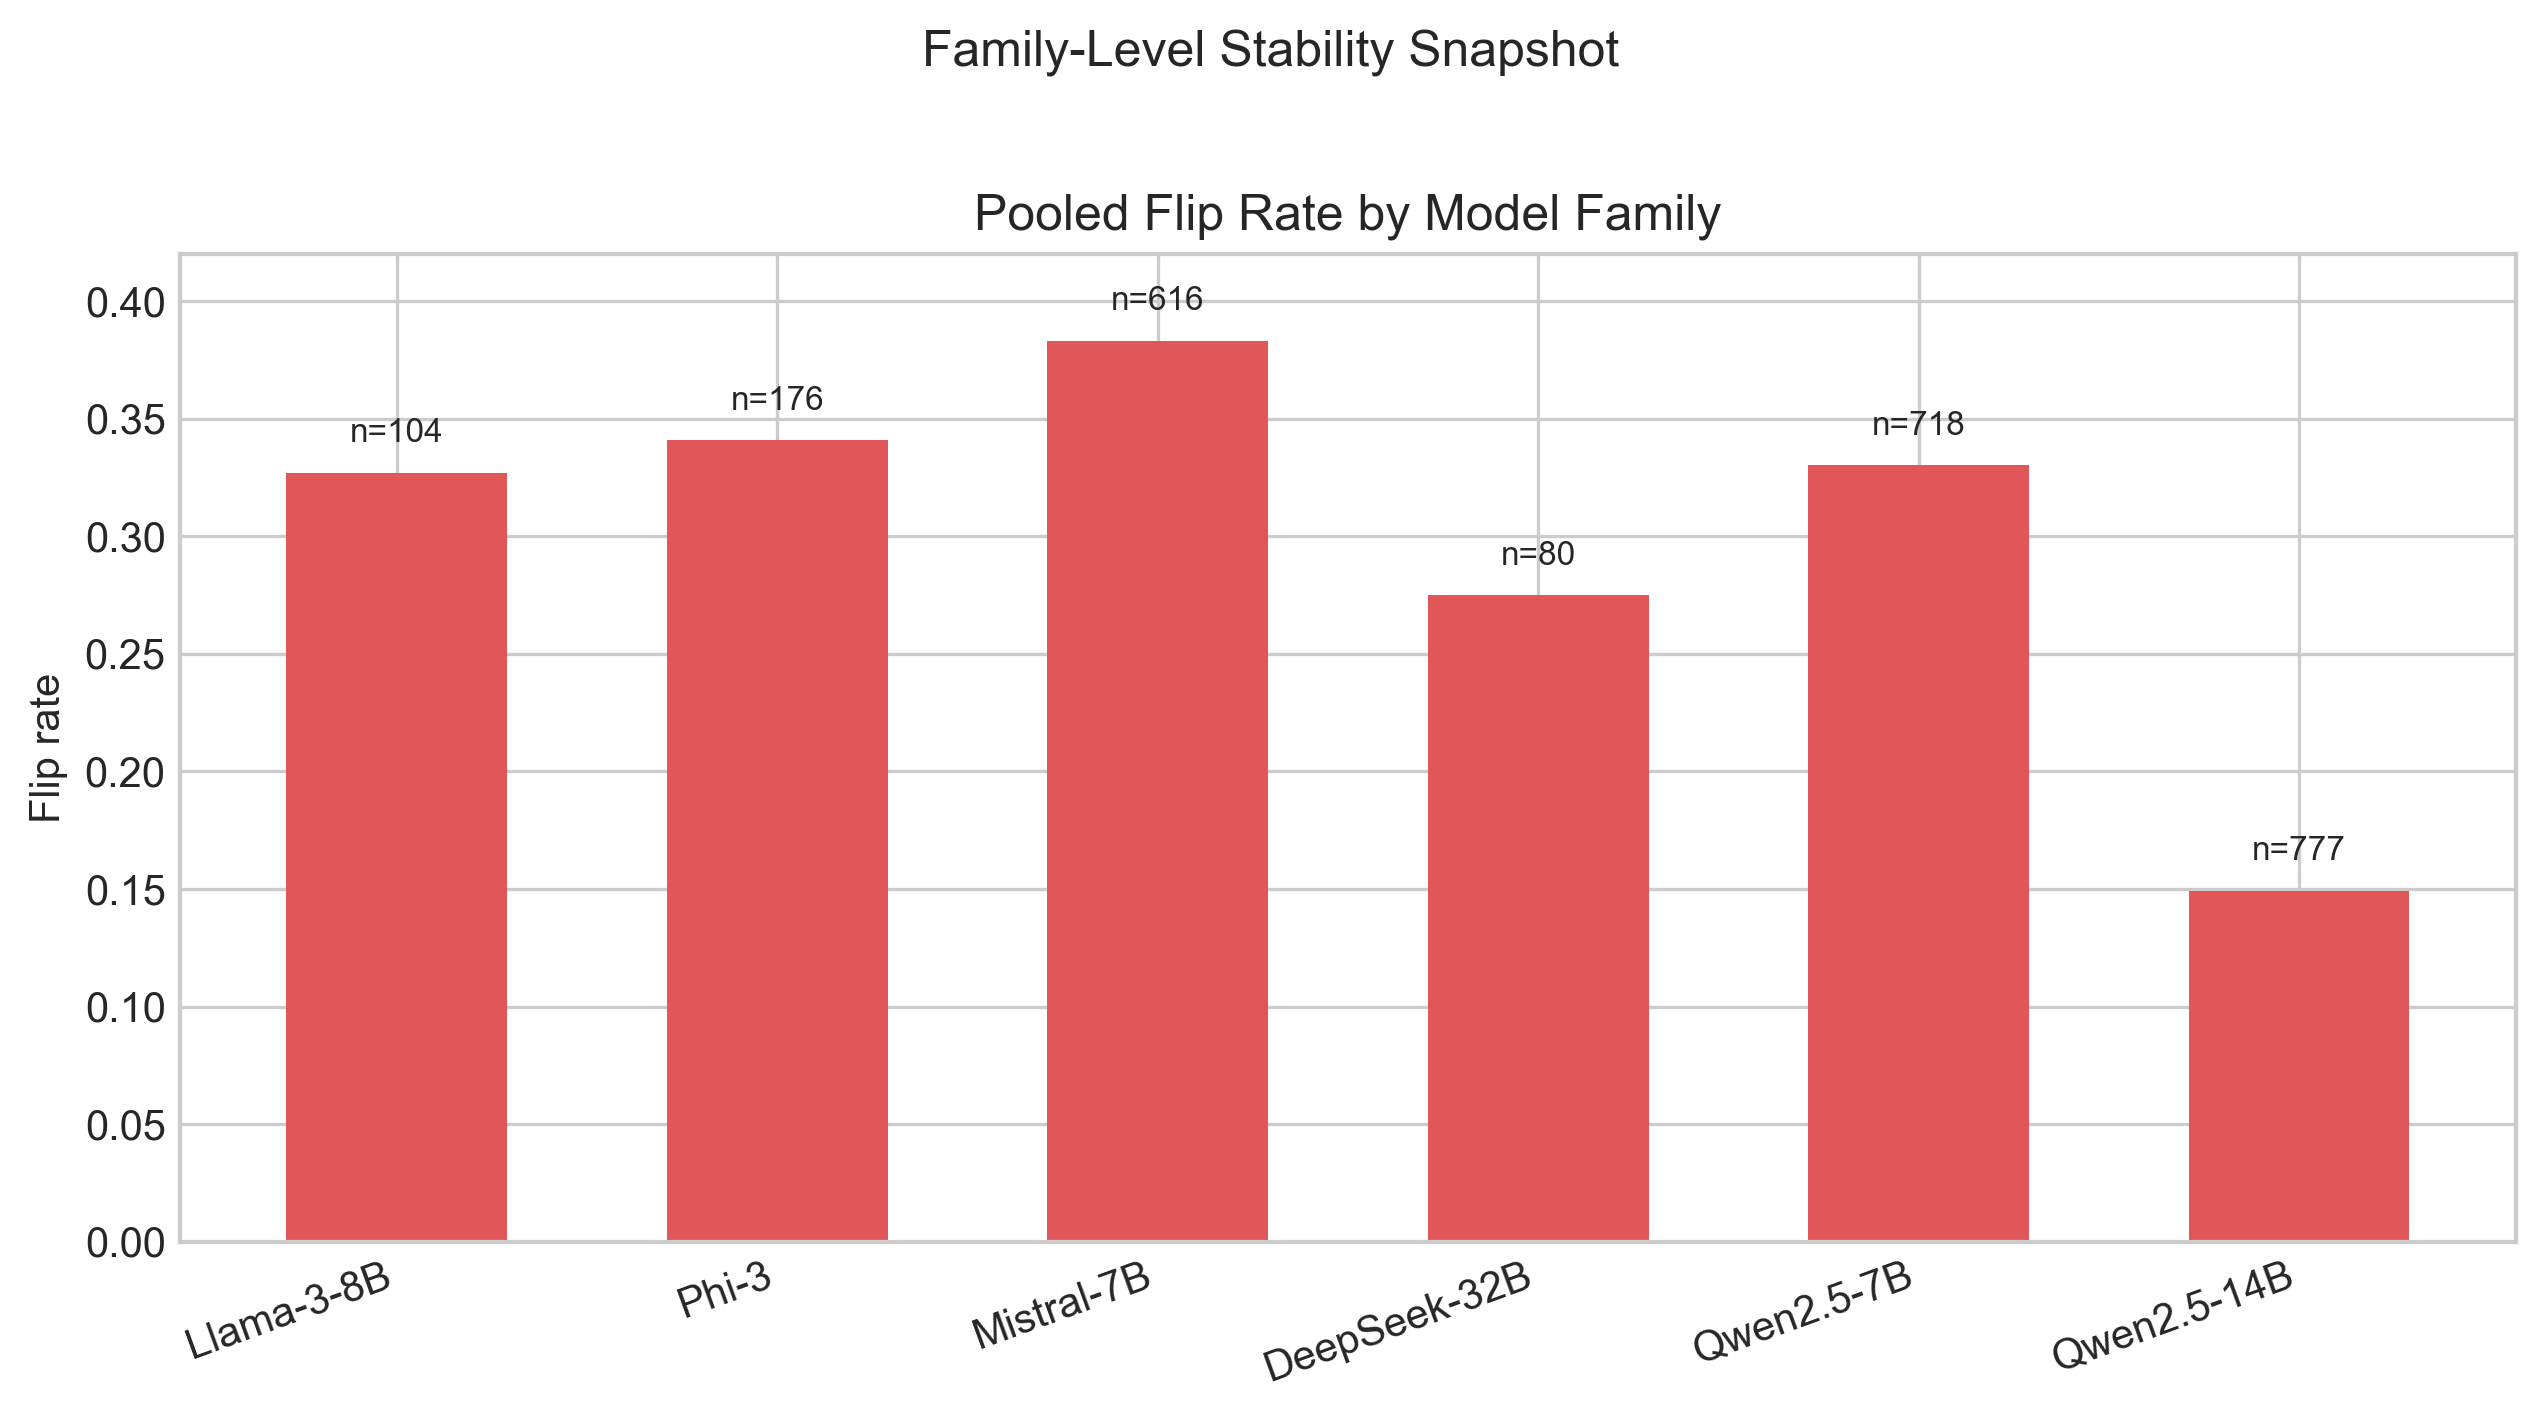
\includegraphics[width=0.92\textwidth]{plots/family_effect_snapshot.png}
\caption{Family-level stability snapshot. Pooled flip rate is non-zero across families, including Llama, Phi, and DeepSeek, indicating that verdict instability persists even when most pooled directional effects are small in Table~\ref{tab:cross_model_snapshot}.}
\label{fig:family_effect_snapshot}
\end{figure*}

This is why our interpretation tracks \emph{direction and stability} together: near-zero pooled direction does not imply deterministic behavior, and flip-rate instability remains a separate fairness risk.

\subsection{What We Can Claim at This Stage}
Based on the full panel, three claims are defensible. (i) Process and outcome can diverge in the pilot: favorable aggregate outcome direction does not guarantee fair trial dynamics. (ii) At pooled family level, directional effects are mixed but generally modest, with the largest positive shifts in Phi and DeepSeek. (iii) Non-trivial flip rates persist across families, so stability auditing remains necessary even when directional bias is moderate rather than extreme.

% =========================================================
\section{Discussion: Practical Implications}

\textbf{For evaluation practice.} A single aggregate fairness metric is insufficient for legal-use audits. Our results support a minimum audit bundle: paired counterfactual outcomes, procedural indicators, placebo controls, and replication checks. This bundle distinguishes directional bias from stochastic instability.

\textbf{For deployment decisions.} The full panel results do not support broad claims that a model is either ``fair'' or ``unfair'' in isolation. Instead, they support a policy of conditional deployment gates: require stable directional behavior across reruns, require near-null placebo effects, and require no material procedural harms before use in high-stakes legal assistance.

\textbf{For research design.} Coverage matters as much as point estimates. The repo workflow (manifest-based resumption, explicit failure accounting, and pair-complete parsing) enables transparent reporting of what is known, what remains underpowered, and which claims are coverage-limited.

% =========================================================
\section{Ablations and Diagnostics}
\textbf{Blinding Ablation.} Compare $\hat{\beta}_1$ and flip rates with and without judge blinding, and verify that blinding enforcement changes only cue exposure (not case facts). \textbf{Placebo Names.} Compare $\hat{\beta}_1$ and flip rates in same-category placebo swaps; effects should be statistically indistinguishable from zero within the pre-registered threshold. \textbf{Paraphrase Robustness.} Keep effects stable across semantic-equivalent paraphrases and report variance ratios. \textbf{Classifier Calibration.} Report tone-calibration curves and groupwise ECE. \textbf{Interruption Detector.} Report $(\alpha,\beta)$ and corrected rates using~\eqref{eq:me_correction}. Figures/tables are produced by the artifact plotting scripts described in Sec.~IX.

% =========================================================
\section{Threats to Validity}
\label{sec:threats}

\textbf{Construct Validity.} Byte share, objections, and tone are proxies rather than direct legal-harm measures; we mitigate this with blinding/placebos and calibration checks. \textbf{Leakage.} Counsel strategy and prompt dynamics may still correlate with cues despite pairing; trial-level blocking and blinding reduce but do not eliminate this risk. \textbf{Provider Drift.} Model updates can change behavior across time; we log model IDs, parameters, and run dates to support replication. \textbf{Case Realism.} Intentionally simple cases improve identification but limit external validity to real legal proceedings.

% =========================================================
\section{Ethical Considerations}

Demographic cueing risks harmful content. We restrict this work to offline audits; cues would be disabled in any production deployment. We limit transcript release, apply safety filtering, and supply usage guidance to reduce misuse risk.

% =========================================================
\section{Reproducibility and Artifact}

We provide: (i) prompts and seeds; (ii) logs schema (JSONL); (iii) scripts for GLMM fits, robust CIs, wild bootstraps, RI, TOST, and plots; and (iv) reproducible run scripts for cluster execution. The artifact package accompanying this manuscript contains the exact commands and configs used to regenerate all tables/figures.

% =========================================================
\section{Conclusion}

\emph{B.A.I.L.I.F.F.} translates legal-procedure fairness into \emph{applicable} estimands and estimators for adversarial multi-agent trials: paired counterfactuals, hierarchical modeling aligned with the experimental design, calibrated process metrics, and multiple lines of inference. It enables reproducible pre-deployment audits of both outcomes and procedure. As legal AI systems move from assistive tooling toward consequential decision support, this style of audit is necessary to enforce procedural justice rather than statistical appeasement.

% =========================================================
% Optional appendix for operational details (kept out of main narrative)
\appendices
\section{Artifact \& Orchestration (Operational)}
\textbf{Endpoints.} We pin provider endpoints by model IDs and log response metadata. \textbf{Scheduling.} Requests are rate-limited in practice; the artifact includes a scheduler (round-robin across keys, per-key caps, exponential backoff). \textbf{Determinism.} Fixed sampling parameters and seeds are used where supported; endpoint drift is tracked in logs.

% ================= Bibliography =================
\balance
\bibliographystyle{IEEEtran}
\begin{thebibliography}{99}

\bibitem{katz2017general}
D.\,M. Katz, M.\,J. Bommarito II, and J. Blackman,
``A general approach for predicting the behavior of the Supreme Court of the United States,''
\emph{PLOS ONE}, vol.~12, no.~4, 2017.

\bibitem{barocas2016big}
S. Barocas and A.\,D. Selbst,
``Big data's disparate impact,''
\emph{California Law Review}, vol. 104, pp. 671--732, 2016.

\bibitem{shah2020predictive}
N. Shah, D. Lv, and A. Ng,
``Predictive bias in AI systems,''
\emph{Nature Machine Intelligence}, vol.~2, no.~8, pp. 456--464, 2020.

\bibitem{blodgett2020language}
S.\,L. Blodgett, S. Barocas, H. Daum\'e III, and H. Wallach,
``Language (technology) is power: A critical survey of bias in NLP,''
in \emph{Proc. ACL}, 2020, pp. 5454--5476.

\bibitem{angwin2016machine}
J. Angwin, J. Larson, S. Mattu, and L. Kirchner,
``Machine bias,''
\emph{ProPublica}, May 23, 2016.

\bibitem{dressel2018accuracy}
J. Dressel and H. Farid,
``The accuracy, fairness, and limits of predicting recidivism,''
\emph{Science Advances}, vol.~4, no.~1, 2018.

\bibitem{starke2022fairness}
C. Starke, J. Baleis, B. Keller, and F. Marcinkowski,
``Fairness perceptions of algorithmic decision-making: A systematic review,''
\emph{Big Data \& Society}, vol.~9, no.~2, 2022.

\bibitem{caliskan2017semantics}
A. Caliskan, J.\,J. Bryson, and A. Narayanan,
``Semantics derived automatically from language corpora contain human-like biases,''
\emph{Science}, vol. 356, no. 6334, pp. 183--186, 2017.

\bibitem{henderson2023trial}
P. Henderson, K. Sucholutsky, and R. Chandra,
``Trial by AI: Examining automated legal decision-making systems,''
\emph{Artificial Intelligence and Law}, vol.~31, no.~2, pp. 245--272, 2023.

\bibitem{yue2025maser}
S. Yue \emph{et al.},
``Multi-Agent Simulator Drives Language Models for Legal Intensive Interaction,''
arXiv:2502.06882, 2025.

\bibitem{xu2024agentcourt}
H. Xu \emph{et al.},
``AgentCourt: Simulating Court with Adversarial Evolvable Lawyer Agents,''
arXiv:2408.08089, 2024.

\bibitem{tyler1988social}
T.\,R. Tyler and E.\,A. Lind,
``A relational model of authority in groups,''
\emph{Advances in Experimental Social Psychology}, vol.~25, pp. 115--191, 1988.

\bibitem{grgic2018human}
H. Grgi\'c-Hlaca, M.\,B. Zafar, K.\,P. Gummadi, and A. Weller,
``The case for process fairness in learning: Feature selection for fair decision making,''
in \emph{NIPS Workshop on Machine Learning and the Law}, 2018.

\bibitem{khan2024adversarial}
Z. Khan \emph{et al.},
``Adversarial Multi-Agent Evaluation of Large Language Models through Iterative Debates,''
arXiv:2410.04663, 2024.

\bibitem{greenwald1995implicit}
A.\,G. Greenwald and M.\,R. Banaji,
``Implicit social cognition: attitudes, self-esteem, and stereotypes,''
\emph{Psychological Review}, vol. 102, no.~1, pp. 4--27, 1995.

\bibitem{bertrand2004emily}
M. Bertrand and S. Mullainathan,
``Are Emily and Greg more employable than Lakisha and Jamal? A field experiment on labor market discrimination,''
\emph{American Economic Review}, vol.~94, no.~4, pp. 991--1013, 2004.

\bibitem{pager2003mark}
D. Pager,
``The mark of a criminal record,''
\emph{American Journal of Sociology}, vol. 108, no.~5, pp. 937--975, 2003.

\bibitem{fryer2004causes}
R.\,G. Fryer Jr and S.\,D. Levitt,
``The causes and consequences of distinctively black names,''
\emph{The Quarterly Journal of Economics}, vol. 119, no.~3, pp. 767--805, 2004.

\bibitem{labov2006social}
W. Labov,
\emph{The Social Stratification of English in New York City}, 2nd~ed.,
Cambridge University Press, 2006.

\bibitem{kleinberg2016inherent}
J. Kleinberg, S. Mullainathan, and M. Raghavan,
``Inherent trade-offs in the fair determination of risk scores,''
arXiv:1609.05807, 2016.

\bibitem{corbett2017algorithmic}
S. Corbett-Davies, E. Pierson, A. Feller, S. Goel, and A. Huq,
``Algorithmic decision making and the cost of fairness,''
in \emph{Proc. KDD}, 2017, pp. 797--806.

\bibitem{gelman2006data}
A. Gelman and J. Hill,
\emph{Data Analysis Using Regression and Multilevel/Hierarchical Models}.
Cambridge University Press, 2006.

\bibitem{rogers2020primer}
A. Rogers, O. Kovaleva, and A. Rumshisky,
``A primer in BERTology: What we know about how BERT works,''
\emph{Transactions of the ACL}, vol.~8, pp. 842--866, 2020.

\end{thebibliography}

\balance
\end{document}
